\section{Algorithm Optimization} \label{sec:algorithm}

\subsection{Adjacency Filtering} \label{sec:af} 

mrFAST suffers from long execution time for several reasons. One of the biggest
reasons is that the edit-distance calculation is time consuming. The other
reason is that the hash-table is not balanced. By time consuming we mean for
each edit-distance calculation, not only computational cost is high, but also
that involves 1 memory lookup to reference DNA data base, which is costly. By
not balanced we mean some patterns store more coordinates within its entry
whereas some patterns store fewer coordinates. For those patterns storing long
lists of coordinates, we call them expensive keys. Expensive keys imply two
problems: 1. Expensive keys have long coordinate list, which means if ever
used them as keys, they will impose many string comparisons and hence many
reference DNA database accesses. 2. In real test cases, they will be
frequently encountered. This property is associated to the first property.
they are popular in human DNA so that they have longer coordinate list. As a
result, when sampling, we will have higher chance encounter these expensive
keys since they show up more frequently in human DNA. \\
 
%%%%%%%%%%%%%%%%%%%%%%%%%%%%%%%%%%%%%%%%%%%%%%%%%%%%%%%%%%%%%%%%%%%%%%%%%%%%%%%%
\begin{figure}[t] 
\centering
\vspace{0.1in}
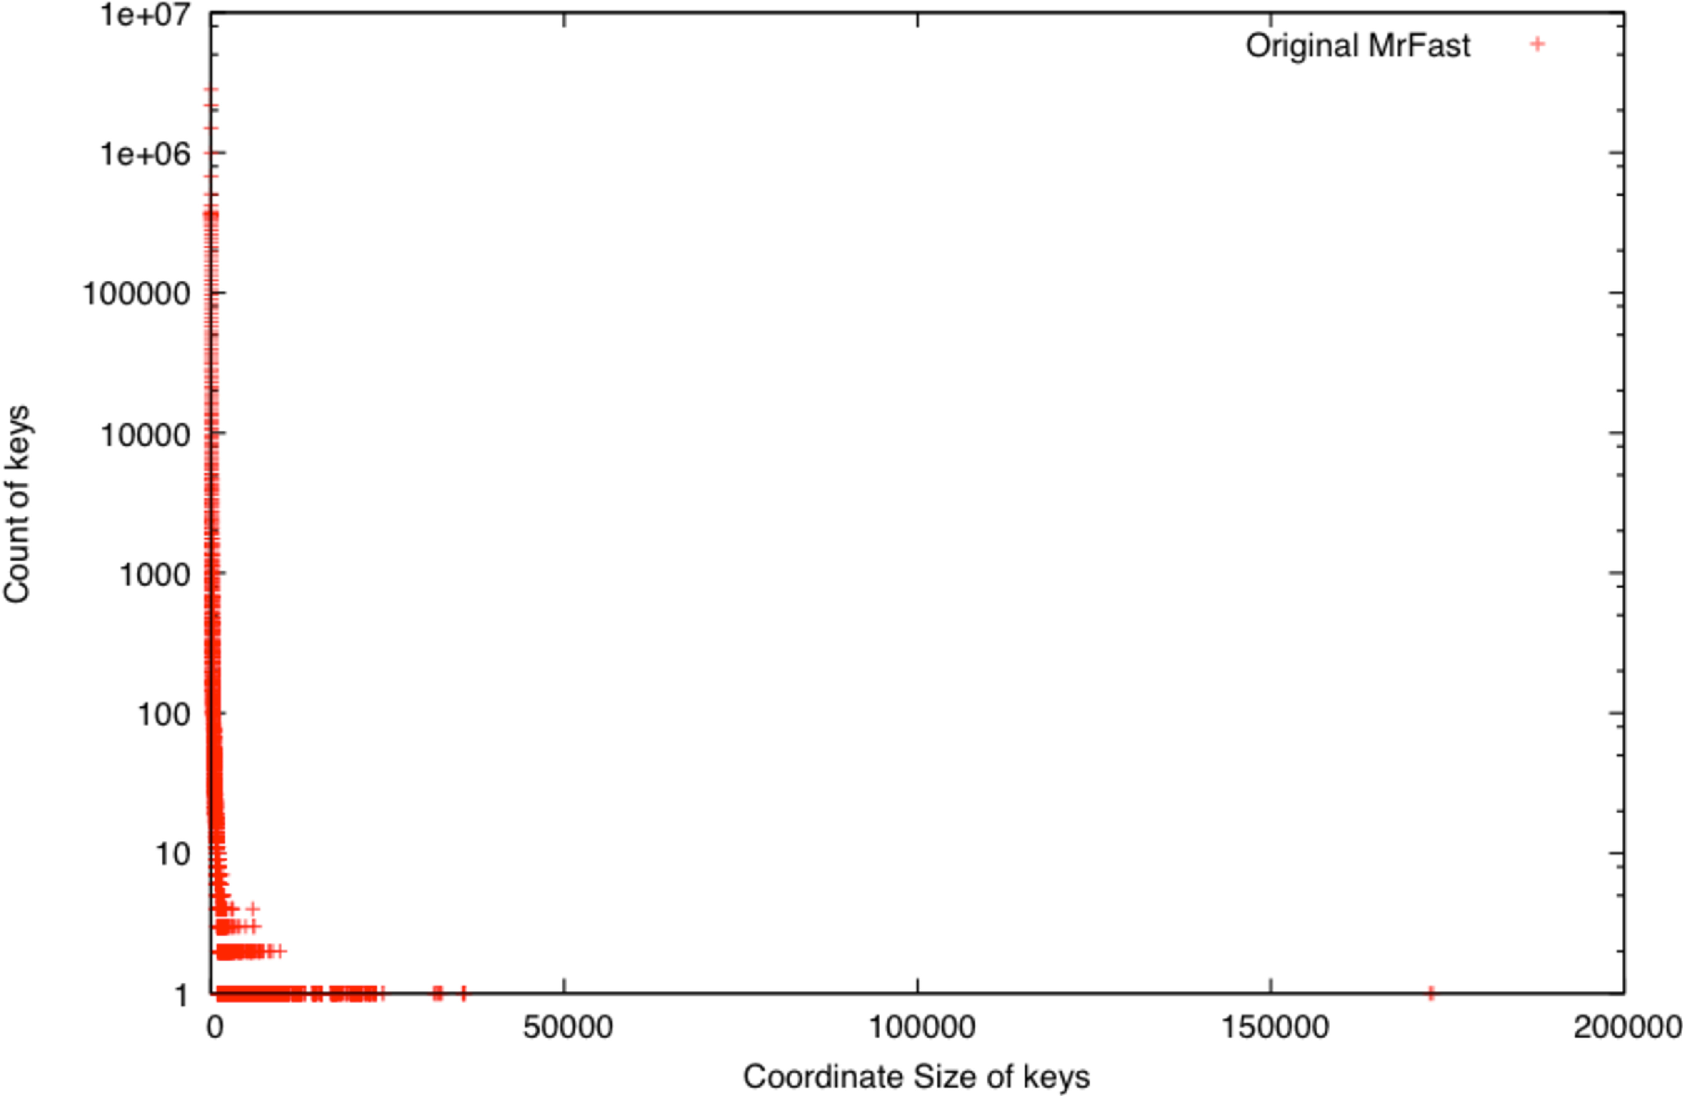
\includegraphics[width=3in]{./figure/Entry_Size_B.pdf} \vspace{0in}
\caption{The coordinate entry size}
\label{fig:entry_size} 
\end{figure}
%%%%%%%%%%%%%%%%%%%%%%%%%%%%%%%%%%%%%%%%%%%%%%%%%%%%%%%%%%%%%%%%%%%%%%%%%%%%%%%%

Figure~\ref{fig:entry_size} shows the coordinates entry size for first chromosome.
For a vast majority of the entries, there is 0 coordinate stored inside which
means this pattern never shows up in this chromosome. However, there are also
some coordinates having more than thousands or even millions of coordinates. As
a result, whenever mrFAST uses those segments as keys, there will be thousands
to millions of edit-distance conducted. Figure~\ref{fig:edit_dist} shows how many
edit-distance calculations performed turned out to be a match. When aligning 10
million fragments from chromosome 1 to chromosome 1, allowing max error number
to be 3 normally out of 3000 edit-distance calculations, 1 will be a match.
Such low matching rate implies that the majority of the coordinates subject to
edit-distance calculation will be rejected, at a high execution time cost.
From our analysis, it turns out some of the not matching coordinates can be
rejected solely by analyzing the information from the hash table alone, without
even accessing reference sequence database and performing the expensive
edit-distance calculation. Such early stage rejection would save memory
bandwidth, on chip cache as well as execution time.\\

%%%%%%%%%%%%%%%%%%%%%%%%%%%%%%%%%%%%%%%%%%%%%%%%%%%%%%%%%%%%%%%%%%%%%%%%%%%%%%%%
\begin{figure}[t] 
\centering
\vspace{0.1in}
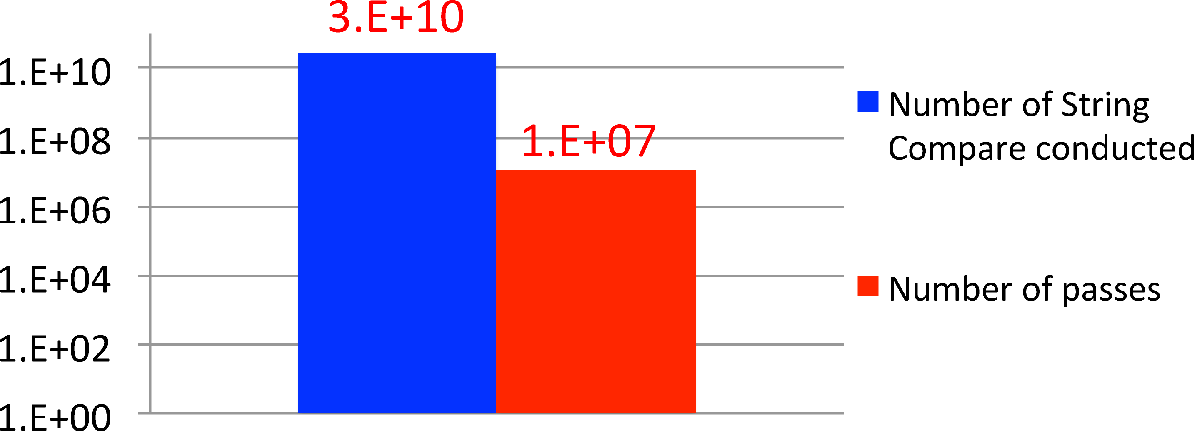
\includegraphics[width=3in]{./figure/Edit_Perform_B.pdf} \vspace{0in}
\caption{The number of edit-distance performs and pass}
\label{fig:edit_dist} 
\end{figure}
%%%%%%%%%%%%%%%%%%%%%%%%%%%%%%%%%%%%%%%%%%%%%%%%%%%%%%%%%%%%%%%%%%%%%%%%%%%%%%%%

The key observation behind this early rejection is that: if the fragment can be
divided into \textit{N} segments, and we probe \textit{e+1} segments'
coordinate lists as we described in section~\ref{hash_query}. Then for each
coordinate stored in the coordinate list, if such coordinate is a potential
match, the adjacent keys should have adjacent locations stored in their
coordinate lists. An example will be the best explanation. For instance, as
shown in Figure~\ref{fig:ad_1}, a fragment f is divided into \textit{N}
segments \textit{s1, s2… sN,} with each segments being \textit{L} in length.
When probing the coordinate entry for the first segment, on the first
coordinate coor1 from \textit{s1}, we test if \textit{coor1 + L} is located in
the coordinate list of \textit{s2} and if \textit{coor1 + 2*L} is located in
the coordinate list of \textit{s3}, so on and so forth. For a perfect match,
all adjacent segments should locate at corresponding locations, which means all
corresponding locations should be stored inside the corresponding coordinate
list. However, for inexact matches, where we allow mismatches, the constrain
will be relaxed to at least \textit{N - e} segments should find corresponding
locations in their coordinate list. The reasons why we relax the filtering
constrain from all segments to \textit{N - e} segments is that now there could
be at most errors in the fragment, which in the worst case could be distributed
in e segments. In presents of insertion and deletions, the filtering test will
be further relaxed to the range of expected coordinate plus or minus
\textit{e}. For example in Figure~\ref{fig:ad_2}, if now the error
number \textit{e} is set to 3, then for \textit{coor1}, instead of searching
for \textit{coor1 + L} in the coordinate list of \textit{s2}, we now search for
\textit{coor1 + L +/- e} for \textit{s2} and \textit{coor1 + L*2 +/- e} for
\textit{s3}, so on and so forth. Additionally, instead of requiring matches for
all of the segments, the fragment will pass the filtering test if more than
\textit{N - e} segments found corresponding locations. \\

%%%%%%%%%%%%%%%%%%%%%%%%%%%%%%%%%%%%%%%%%%%%%%%%%%%%%%%%%%%%%%%%%%%%%%%%%%%%%%%%
\begin{figure}[t] 
\centering
\vspace{0.1in}
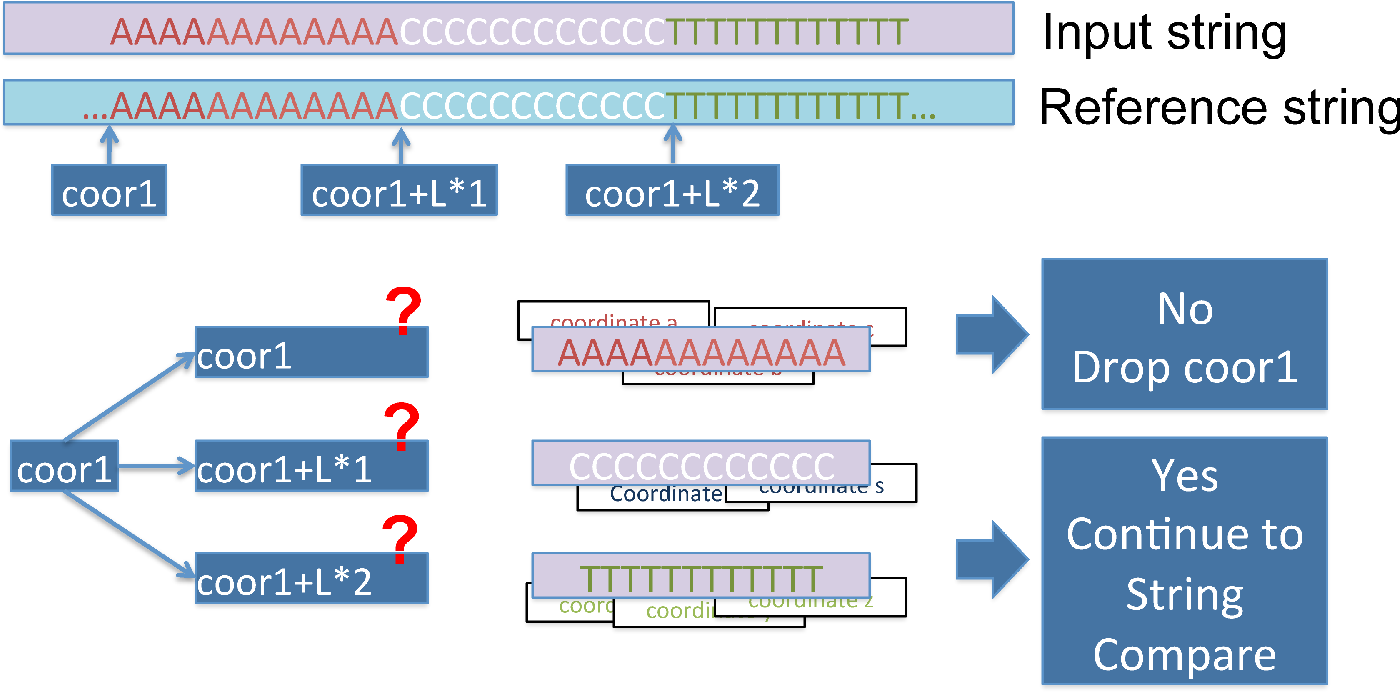
\includegraphics[width=3in]{./figure/AD_1_B.pdf} \vspace{0in}
\caption{Adjacency Filtering for exact match}
\label{fig:ad_1} 
\end{figure}
%%%%%%%%%%%%%%%%%%%%%%%%%%%%%%%%%%%%%%%%%%%%%%%%%%%%%%%%%%%%%%%%%%%%%%%%%%%%%%%%

Adjacency Filtering itself will not guarantee matches but it will filter out
obvious not matching locations. If a fragment has more than \textit{N - e}
segments that fail finding adjacent coordinates, we can deduce there must be
more than \textit{e} errors thus rejecting the coordinate. However, if the
fragment passes the adjacency filtering, this does not necessarily mean the
input fragment matches to the reference DNA sequence within \textit{e} errors.
We cannot guarantee the total error number is less than \textit{e} since for
those segments that failed finding adjacent locations in their coordinate
lists, they might have more than 1 errors in it. Thus by the Adjacency
Filtering itself is not complete. For a matching input fragment and reference
DNA coordinate pair that passes adjacency filtering process, we still have to
perform edit distance calculation on them to get the exact number and locations
of the errors. Although adjacency filtering is not complete and cannot replace
edit-distance calculation, it did drastically reduced the times of
edit-distance being called. We will show the numbers in evaluation section.\\

%%%%%%%%%%%%%%%%%%%%%%%%%%%%%%%%%%%%%%%%%%%%%%%%%%%%%%%%%%%%%%%%%%%%%%%%%%%%%%%%
\begin{figure}[t] 
\centering
\vspace{0.1in}
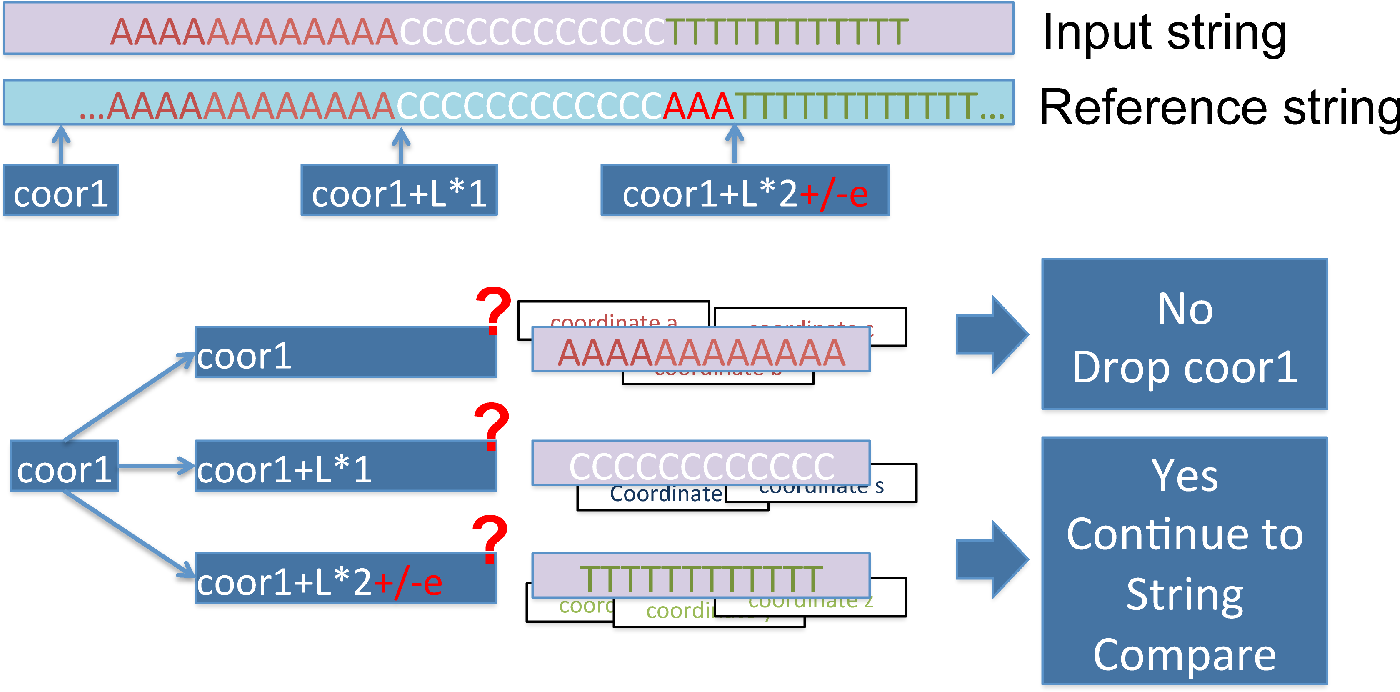
\includegraphics[width=3in]{./figure/AD_2_B.pdf} \vspace{0in}
\caption{Adjacency Filtering for inexact match}
\label{fig:ad_2} 
\end{figure}
%%%%%%%%%%%%%%%%%%%%%%%%%%%%%%%%%%%%%%%%%%%%%%%%%%%%%%%%%%%%%%%%%%%%%%%%%%%%%%%%

\subsection{Cheap Key Selection} \label{sec:cheapkey}

\subsubsection{Pigeon Hole theorem and multiple search keys} 

There are several reasons why we have to allow several errors for finding out
potential matching locations. First is the potential difference between
individual DNA sequences. Most portion of individual DNA sequence is similar
with reference DNA sequences and using this similarity, we have tried to
reconstruct individual DNA sequences by matching it to the known reference
sequences. However, most of important things is to find differences between
input fragments and reference DNA sequence. These differences can cause specific
diseases or determine specific individual characteristics. So, one of the most
important thing for matching fragment to reference sequence is to give the
potential location within maximum allowable errors, such as insertion, deletion
and mismatch. Second reason is that there are potential errors caused by DNA
sequencing analyzer’s misreading. For example, Illumina platform has relatively
poor performance in assorting G-C, i.e. Illumina platform frequently misread G
as C or vice versa. The other NGS platforms also have their own sequencing
biases. By matching fragments to reference sequence with allowing specific
number of errors, we can reduce the matching failures caused by NGS platforms
specific errors. String comparison operation of mrFAST can give the
edit-distance between two sequences, which can be the threshold values to decide
whether the location can be the potential location of fragment or not. However,
main assumption of hash table based seed-and-extend algorithm is that there is
no error in the fragment of key. If we assume that the fragment has some errors
caused by a certain reason, like individual DNA difference or platform biases,
and the errors are located at the searching key for hash table, then, the
coordinates according to the search key have potential errors. Finally, we lose
the chance that we can find out exact matching cases with allowing these
errors.\\

The obvious solution of this potential problem is to select multiple search keys
within the fragment, which is based on Pigeon Hole theorem. Pigeon Hole theorem
is that if there are \textit{m} pigeon and \textit{m+1} hole which can be
occupied by just one pigeon, then at least one of the keys will not have errors.
If \textit{m+1} keys are selected as search key to guarantee \textit{m}
allowable errors, then, one of the search keys don’t has errors at least.
Figure~\ref{fig:pigeon} shows the worst case of error distribution. 5 errors
distributed across the different keys. In this case, if we select any 6 keys of
total keys, we can get a key which do not has errors at least. 

%%%%%%%%%%%%%%%%%%%%%%%%%%%%%%%%%%%%%%%%%%%%%%%%%%%%%%%%%%%%%%%%%%%%%%%%%%%%%%%%
\begin{figure}[b] \centering \vspace{0.1in}
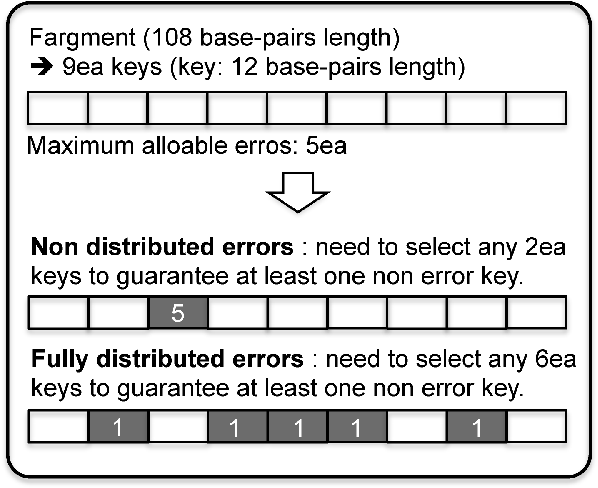
\includegraphics[width=2.5in]{./figure/pigeon_B.pdf} \vspace{0in}
\caption{Error distribution \& required number of keys}
\label{fig:pigeon} 
\end{figure}
%%%%%%%%%%%%%%%%%%%%%%%%%%%%%%%%%%%%%%%%%%%%%%%%%%%%%%%%%%%%%%%%%%%%%%%%%%%%%%%%

\subsubsection{Avoid duplicated Adjacency filtering at using multiple searching keys}

When we try to use \textit{e+1} keys as searching keys of Adjacency Filtering,
if the fragment is passed, then, it is possible that there are duplicated
Adjacency Filtering computations. For example, if the fragment is exactly
matched to the reference sequence at certain coordinate and we selected
\textit{e+1} keys as searching keys, then, each Adjacency Filtering
corresponding to \textit{e+1} keys find out same coordinate as potentially
matching coordinate. This means that \textit{e+1} duplicated Adjacency
Filtering operations are computed for finding out just one possible location.
We can filter out these duplicated and redundant Adjacency operations by
comparing the expected coordinate as the result of Adjacency filtering and the
coordinates, already found as potentially matching coordinate before taking
Adjacency filtering. We preserve the potentially matching coordinates, the
result of previous Adjacency Filtering at specific sized, 100ea in our
implementation, array to filter out the redundant Adjacency filter. If it is
matched, then, we simply cancel the reserved Adjacency Filtering.

%%%%%%%%%%%%%%%%%%%%%%%%%%%%%%%%%%%%%%%%%%%%%%%%%%%%%%%%%%%%%%%%%%%%%%%%%%%%%%%%
\begin{figure}[t] \centering \vspace{0.1in}
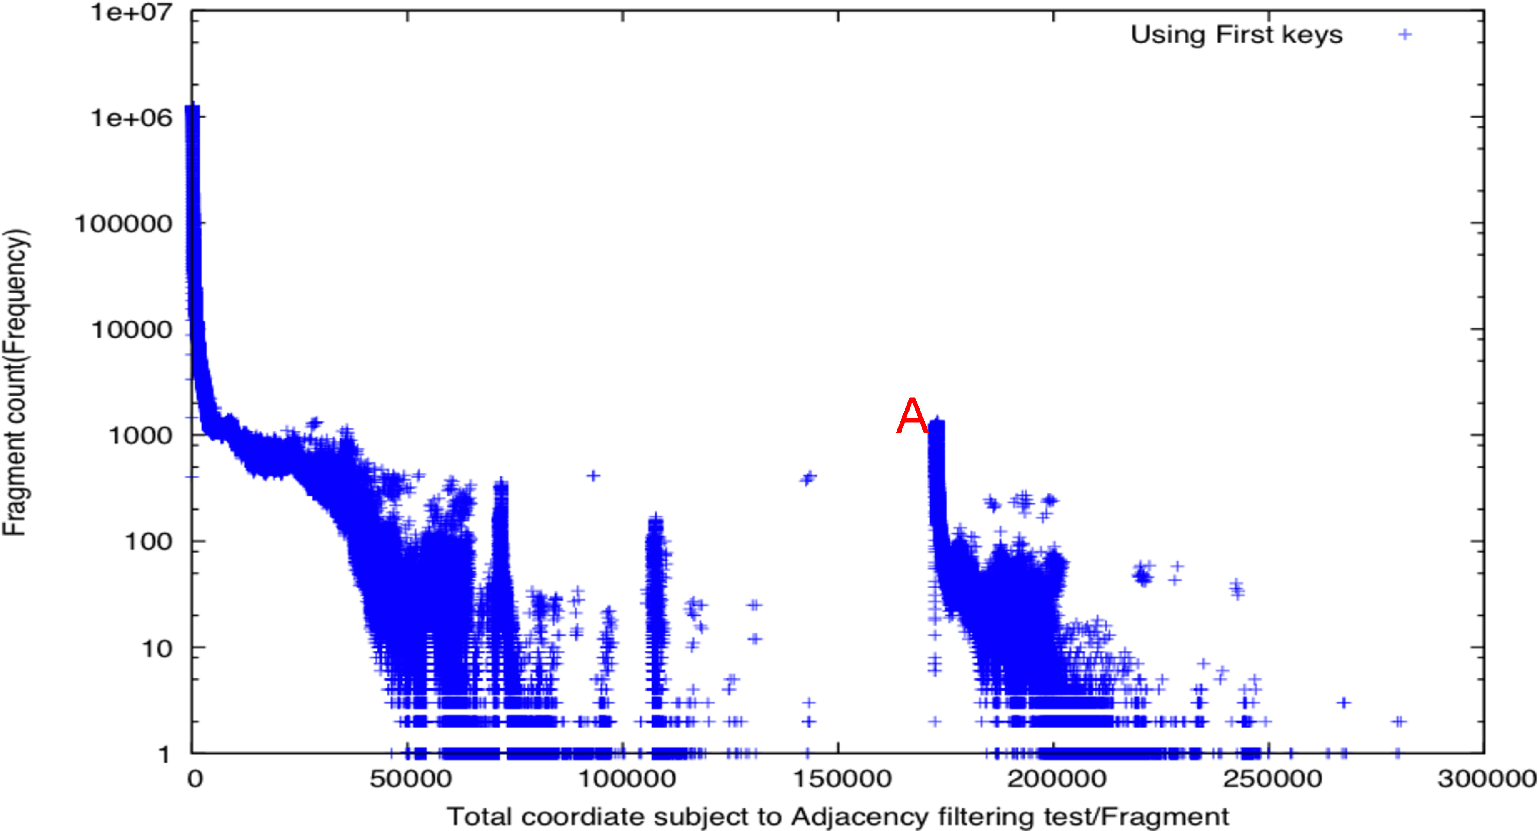
\includegraphics[height=1.7in]{./figure/Key_Dist_B.pdf} \vspace{0in}
\caption{Adjacency Filtering Distribution} 
\label{fig:key_dist} 
\end{figure}
%%%%%%%%%%%%%%%%%%%%%%%%%%%%%%%%%%%%%%%%%%%%%%%%%%%%%%%%%%%%%%%%%%%%%%%%%%%%%%%%

\subsubsection{Imbalance of the number of key entry size} 

In section~\ref{sec:af}, Adjacency filtering drastically reduces the number of
string comparison perform. However, Adjacency filtering also requires large
computational resources for searching the expected coordinate in hash table to
decide whether this location can be potentially matched to fragment or not. The
imbalance of key entry size exacerbates the problem because we have to perform
Adjacency Filtering as much as key entry size. Figure~\ref{fig:key_dist} shows
the distribution of key entry size within one chromosome. If we use the
fragments which are located at \textit{A} position, about 150,000 Adjacency
Filtering performs are required. The number of fragments located at \textit{A}
position is over 1000. Now, the dominant computation requirement changes from
the string comparison perform to Adjacency Filtering perform.

%%%%%%%%%%%%%%%%%%%%%%%%%%%%%%%%%%%%%%%%%%%%%%%%%%%%%%%%%%%%%%%%%%%%%%%%%%%%%%%%
\begin{figure}[h] \centering \vspace{0.1in}
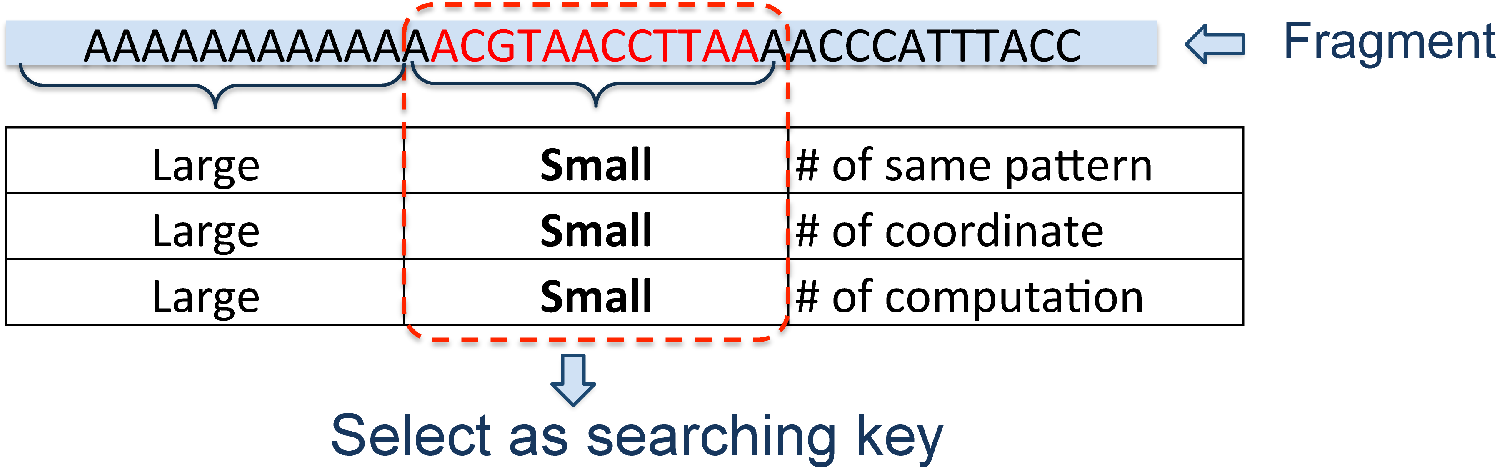
\includegraphics[width=3.0in]{./figure/Cheap_Key_B.pdf} \vspace{0in}
\caption{Cheap Key Selection Mechanism} 
\label{fig:cheap_key} 
\end{figure}
%%%%%%%%%%%%%%%%%%%%%%%%%%%%%%%%%%%%%%%%%%%%%%%%%%%%%%%%%%%%%%%%%%%%%%%%%%%%%%%%
%%%%%%%%%%%%%%%%%%%%%%%%%%%%%%%%%%%%%%%%%%%%%%%%%%%%%%%%%%%%%%%%%%%%%%%%%%%%%%%%
\begin{figure}[b] \centering \vspace{0.1in}
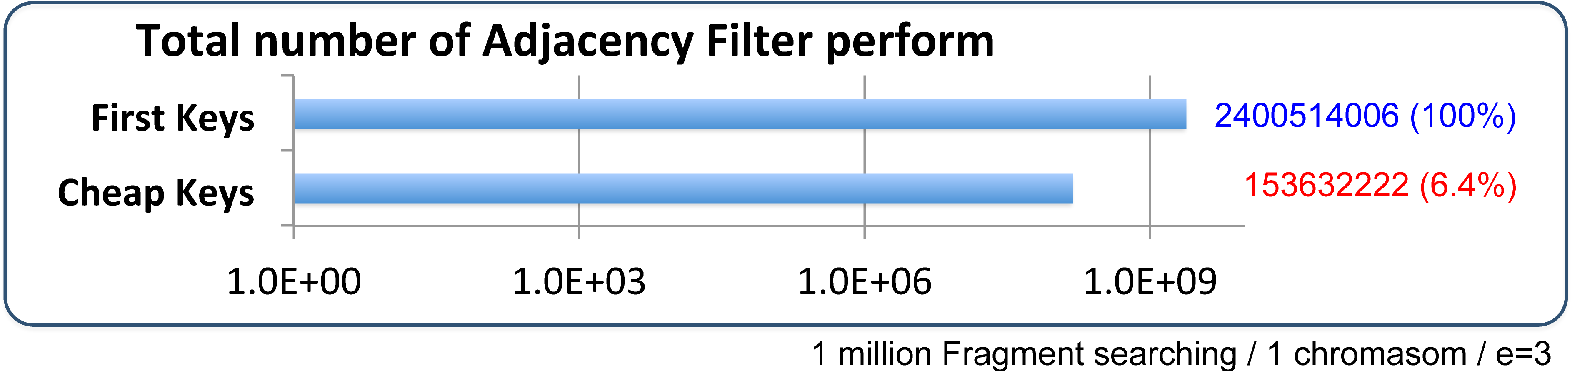
\includegraphics[width=3.0in]{./figure/CK_Result_B.pdf} \vspace{0in}
\caption{Cheap Key Selection Result} 
\label{fig:ck_result} 
\end{figure}
%%%%%%%%%%%%%%%%%%%%%%%%%%%%%%%%%%%%%%%%%%%%%%%%%%%%%%%%%%%%%%%%%%%%%%%%%%%%%%%%
%%%%%%%%%%%%%%%%%%%%%%%%%%%%%%%%%%%%%%%%%%%%%%%%%%%%%%%%%%%%%%%%%%%%%%%%%%%%%%%%
\begin{figure}[t] \centering \vspace{0.1in}
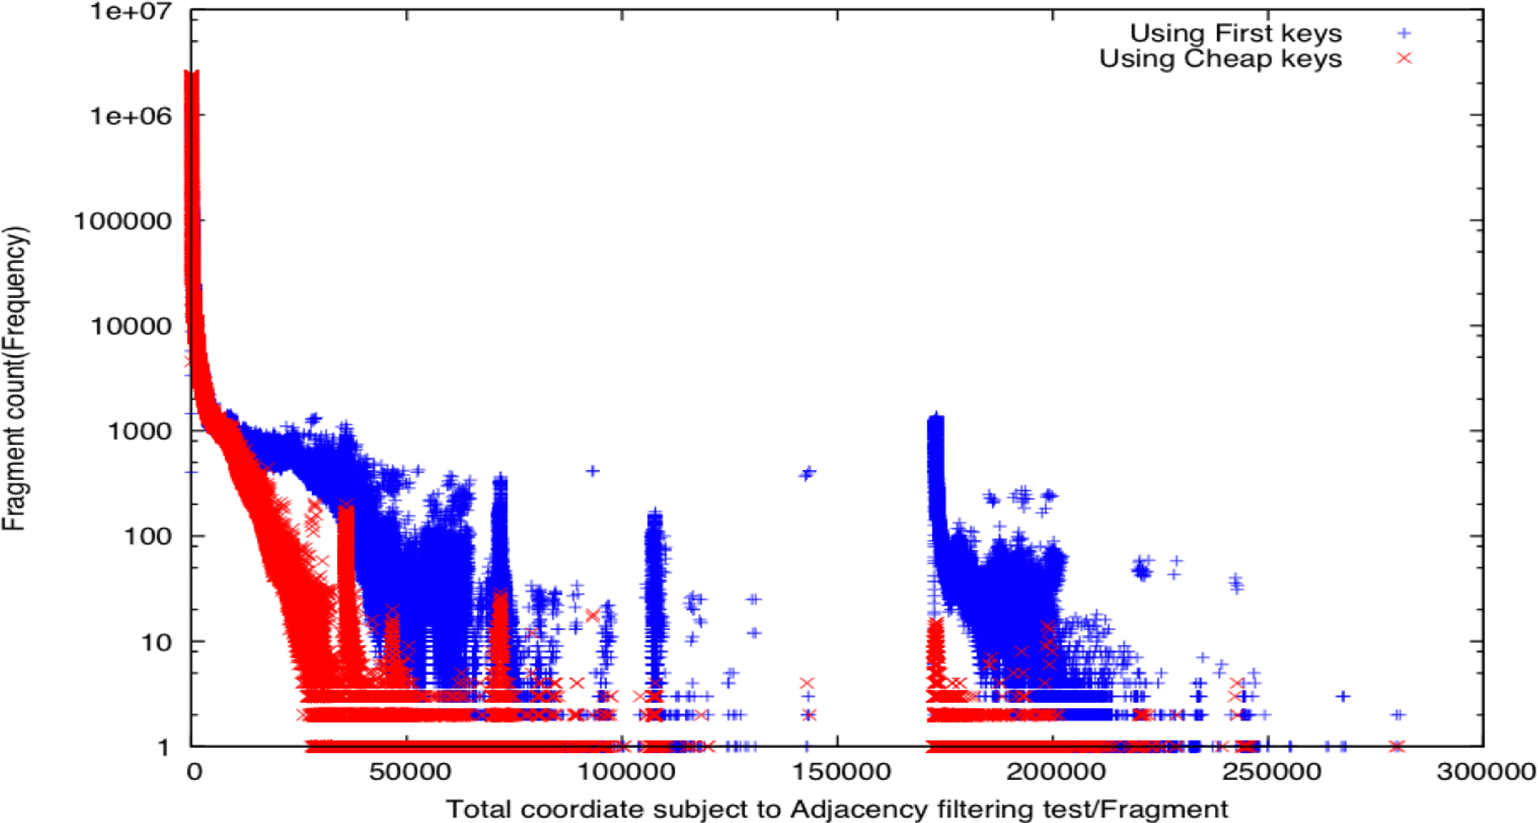
\includegraphics[height=1.7in]{./figure/Key_Dist2_B.pdf} \vspace{0in}
\caption{Efficiency of Cheap Key Selection} 
\label{fig:key_dist2} 
\end{figure}
%%%%%%%%%%%%%%%%%%%%%%%%%%%%%%%%%%%%%%%%%%%%%%%%%%%%%%%%%%%%%%%%%%%%%%%%%%%%%%%%

\subsubsection{Cheap Key Selection} 

If we allow \textit{e} errors, \textit{e+1} searching keys have to be selected
to maintain comprehensiveness. Each key has its own key entry size. To avoid
large Adjacent Filtering computation, we can select the smallest \textit{e+1}
keys as searching keys. Hash table already stores the entry sizes corresponding
to each key and based on this information, we can easily sort the key at the
order of entry size and select cheapest \textit{e+1} keys as searching keys. In
this case, we can drastically reduce the number of Adjacency Filtering
computations and increase the sequencing performance without degrading
comprehensiveness. We call this as Cheap Key Selection.
Figure~\ref{fig:cheap_key} shows the operation of Cheap Key Selection. First of
all, we divide the fragments as keys, i.e. if each fragment has 108ea base
pairs and we use 12ea key length hash table, then we can divide the fragments
as 9 keys. After that, the keys of the fragment can be sorted at the order of
key entry size and cheapest \textit{e+1} keys can be selected as searching
keys. Figure~\ref{fig:key_dist2} shows the efficiency of Cheap Key Selection.
The blue colored diagram represents the original distribution of Adjacency
Filtering and the red colored diagram represents the distribution after Cheap
Key Selection. The number of the fragments, which requires large Adjacency
Filtering perform is drastically reduced. Figure~\ref{fig:ck_result} shows that
the total number of Adjacency Filtering perform is reduced to 6.4\% of original
total number of Adjacency Filtering at the case of selecting first \textit{e+1}
keys as searching keys without sorting based on the entry size. The Cheap Key
Selection also requires computational resources and the number of computations
for sorting is proportional to log (the number of keys within each fragment).
However, the number of Adjacency filtering is proportional to (the number of
keys within fragment) * log (the key entry size). Usually, the fragments have
100 - 200 base pairs and the key length of Hash Table is about 10 to 12, So, the
cost of Cheap Key Selection computation is quite smaller than the cost of
Adjacency Filtering. 
